We note 
        \[f_{\alpha, \beta}^{tr} \sim \text{InvGamma}_{[0, b]}(\alpha, \beta) \quad f_{\alpha, \beta} \sim \text{InvGamma}(\alpha, \beta) \]
        The integral of interest is
        \[\mathbb{E}_{f_Y}\left[ 1 - Y^2 \right] \quad \text{where } Y \sim \text{InvGamma}_{[0, b]}(\alpha, \beta)\]

\begin{answerenum}
    \item If we sample \(X \sim \text{InvGamma}(\alpha, \beta)\), then 
        \[\mathbb{E}_{f_Y}\left[ 1 - Y^2 \right] = \int_{-\infty}^{\infty} (1 - y^2) \frac{f_{\alpha, \beta}(y)}{F_{\alpha, \beta}(b) - F_{\alpha, \beta}(0)} \, dy = \frac{\mathbb{E}_{f_X}\left[ (1 - X^2) \right]}{F_{\alpha, \beta}(b) - F_{\alpha, \beta}(0)} \]

        Thus we can estimate \(\mathbb{E}_{f_Y}\left[ 1 - Y^2 \right]\) by sampling \(X_i \sim \text{InvGamma}(\alpha, \beta)\) and computing
        \[\hat{\theta}_n = \frac{1}{(F_{\alpha, \beta}(b) - F_{\alpha, \beta}(0))n} \sum_{i=1}^n (1 - X_i^2) \]
    \item If we sample \(X \sim \text{InvGamma}_{[0, b]}(\alpha, \beta)\), then
        \[\mathbb{E}_{f_Y}\left[ 1 - Y^2 \right] = \int_0^b (1 - y^2) f_{\alpha, \beta}^{tr}(y) \, dy = \mathbb{E}_{f_X}\left[ 1 - X^2 \right] \]

        Thus we can estimate \(\mathbb{E}_{f_Y}\left[ 1 - Y^2 \right]\) by sampling \(X_i \sim \text{InvGamma}_{[0, b]}(\alpha, \beta)\) and computing
        \[\hat{\theta}_n = \frac{1}{n} \sum_{i=1}^n (1 - X_i^2) \]

    \item The variance and the computation time of the two estimators are compared below for \(b = 0.5, 5\).
\end{answerenum}

\begin{figure}[h]
    \centering
    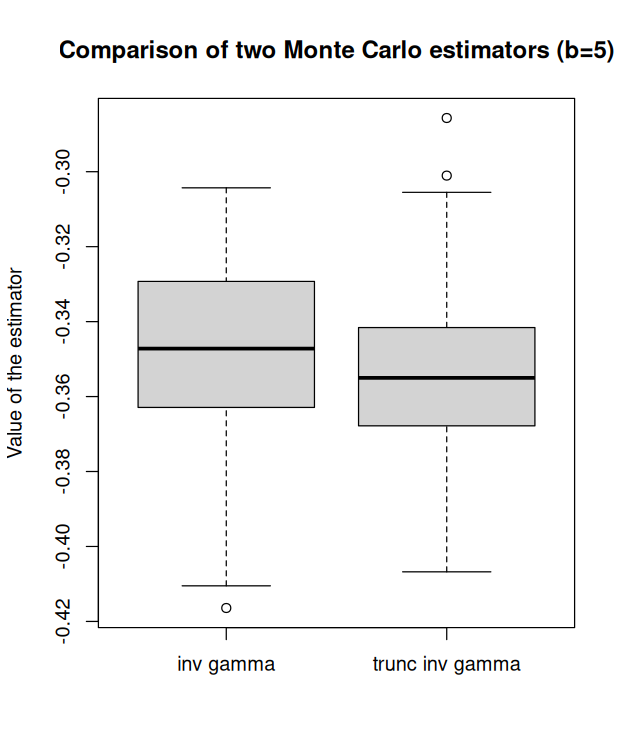
\includegraphics[width=0.22\columnwidth]{imgs/mc_val_bEq5.png}%
    \hspace{0.01\columnwidth}%
    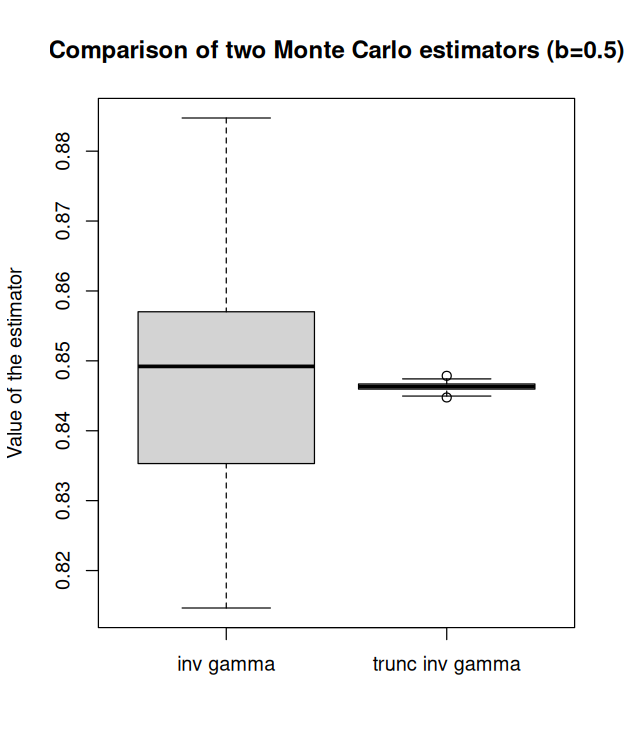
\includegraphics[width=0.22\columnwidth]{imgs/mc_val_bEq05.png}
    \hspace{0.01\columnwidth}
    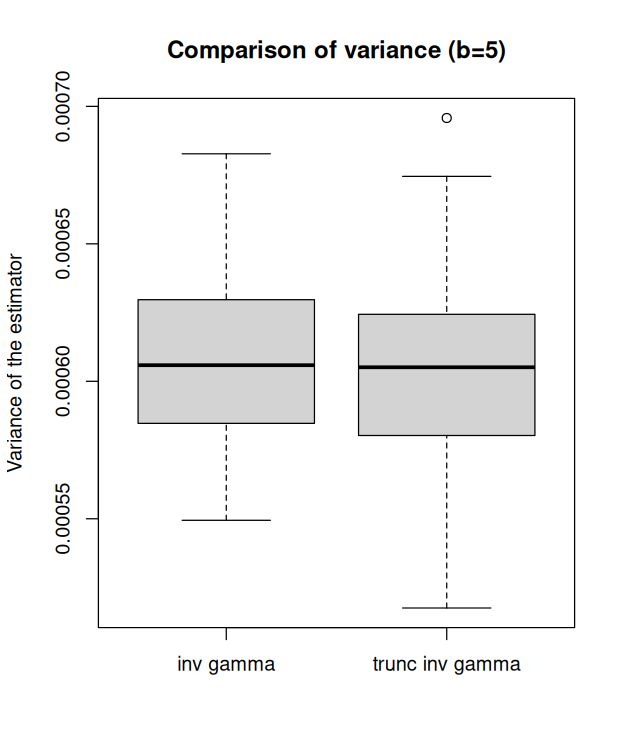
\includegraphics[width=0.22\columnwidth]{imgs/mc_var_bEq5.png}%
    \hspace{0.01\columnwidth}%
    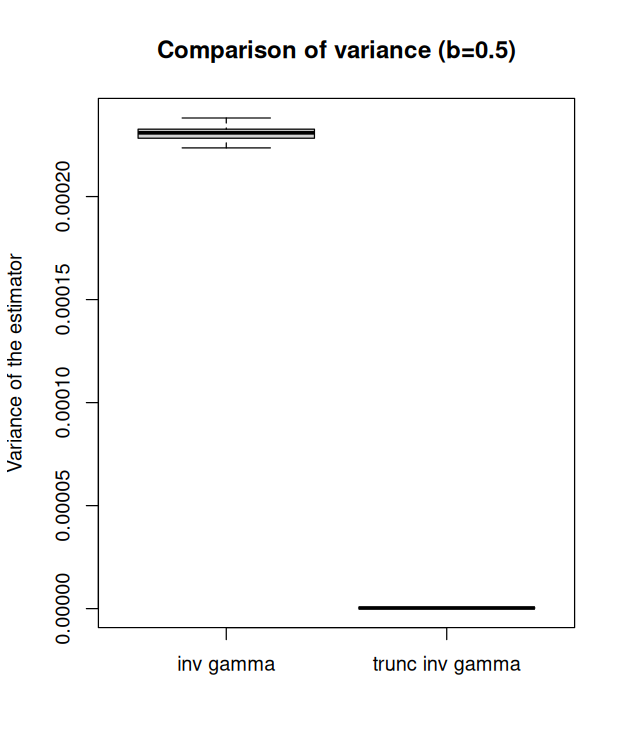
\includegraphics[width=0.22\columnwidth]{imgs/mc_var_bEq05.png}
\end{figure}

From the results, we can see that for \( b = 5\), the two estimators have similar variance, the variance of each estimate is also similarly distributed. However, for the case of \( b = 0.5\), the truncated inverse-gamma based estimator has significantly lower variance compared to the full inverse-gamma based estimator. We figure out that when \(b\) is small, a large portion of the distribution's mass lies outside the truncation interval \([0, b]\). As a result, samples drawn from the full inverse-gamma distribution often fall outside this interval, leading to higher variability in the estimates. In contrast, samples drawn from the truncated inverse-gamma distribution are confined within \([0, b]\), resulting in more consistent and reliable estimates with lower variance.